\documentclass[10pt,a4paper]{article}
\usepackage[utf8]{inputenc}
\usepackage[italian]{babel}
\usepackage{amsmath}
\usepackage{amsfonts}
\usepackage{amssymb}
\usepackage{graphicx}
\usepackage{hyperref}
\usepackage[left=2cm,right=2cm,top=2cm,bottom=2cm]{geometry}
\newcommand{\rem}[1]{[\emph{#1}]}

\author{Belliardo Federico}
\title{Notes on Carroll}
\begin{document}
\maketitle
\begin{itemize}
\item Ragionare sulle diverse formulazioni del principio di equivalenza.
\item Non mi è chiaro l'esempio dell'effetto doppler per chiarire che il tempo scorre a velocità diverse nel campo gravitazionale.

\item p.77 Come si modificano i coni di luce nella metrica di Robertson-Walker se considero anche le altre due coordinate z e y: se le ogni coordinata presenta lo stesso fatto di espansione è sufficiente ruotare la linea 1d ottenuta nel libro.

\item Dimostrare che la derivata covariante (Levi-Civita) del tensore di Levi-Civita è nulla. E che è anche nulla la derivata covariante della metrica inversa.

\textbf{Appunti sulla relatività ristretta}
In relatività ristretta si introduce il concetto di sistema di riferimento inerziale come un insieme di regoli e orologi che costituisco le coordinate cartesiane solidali tra di loro, cioè di modo che un corpo non soggetto a forze si muova i linea retta. In questo sistema di riferimento è data una metrica $\eta_{\mu \nu}$ che per il postulato di invarianza della velocità della luce deve essere conservata inq qualunque altro sistema di riferimento inerziale (stesso cono in cui le forme quadratiche si annullano). Consideriamo le possibili trasformazioni che preservano la caratteristica di essere sistema inerziale, queste sono le trasformazioni lineari. In particolare quelle che preservano anche la metrica si chiamano trasformazioni di Lorentz e sono interpretate come le rotazioni e i boost del sistema di riferimento (dato che contengono 6 parametri liberi). Un altro principio afferma che le leggi della fisica siano le stesse in qualunque sistema di riferimento inerziale ed è per questo che esse sono costruite contraendo tensori di Lorentz. 
Le trasformazioni di Loretz vanno da coordinate cartesiane a coordinate cartesiane e tutto il formalismo è costruito in coordinate cartesiane. Le equazioni di Maxwell in forma classica sono vere per qualunque coordinate (infatti si possono scrivere il gradiente, il rotore e la divergenza in coordinate sferiche, cilidriche, ...). Anche le equazioni in forma covariante (per la relatività ristretta) sono esprimibili in coordinate diverse a patto di trovare l'espressione corretta per la quadridivergenza e il quadrirotore e così via. Essendo una complicazione non necessaria si preferisce pensare alla relatività ristretta come espressa in coordinate cartesiane (dove si passa da un sistema all'altro con una trasformazione di Lorentz, non è vero in generale). I corpi accelerati in ristretta possono essere trattati usando il sistema tangente.
Nella relatività generale le equazioni di Maxwell sono scritte sencondo al prescrizione del minimal coupling come: $\nabla_{a} F^{a b} = 0$ queste sono invarianti per cambi di coordinate generali. In un sistema di riferimento locale inerziale in cui uso coordinate sferiche questa equazione riproduce le classiche equazioni di Maxwell. \textbf{Non c'è alcun contenuto fisico nello scrivere queste equazioni, semplicemente in uno spazio piatto sappiamo che vi è una certa legge tensoriale che sono le equazioni di Maxwell, sappiamo anche che in un sistema di riferimento inerziale $\partial_{\rho} F^{\rho \nu} = 0$, quella scritta è l'unica equazione tensoriale che in un sistema di riferimento inerziale si riduce alla relatività ristretta, quindi se le leggi della fisica sono tensoriali quella è l'unica possibile. Se lo spazio tempo non è piatto potrebbero esserci altri termini che noi non conosciamo poiché  $\partial_{\rho} F^{\rho \nu} = 0$ è una legge per sistemi inerziali in uno spazio piatto.}. Nel sistema di riferimento inerziale locale queste equazioni sono le equazioni di Maxwell ma ora esse sono ben definite in termini tensoriali su tutta la varietà. Quando si fa normale elettromagnetismo o elettrodinamica quantistica si dice che mi metto nel sistema di riferimento inerziale locale in cui la metrica è Minkowski, i coefficienti di Christoffel sono nulli e possono usare le equazioni di maxwell della relatività ristretta. Le trasformazioni di Lorentz portano da sistemi inerziali a altri sistemi inerziali.
Posso pensare alla ordinaria QFT come a una versione della generale QFT in curved space time (in cui le lagrangiane sono invarianti per GCT) in cui lo spazio è piatto, cioè il Riemann si annulla e ho costruito un sistema di riferimento per cui in tutto un'aperto (che è il mio universo) la metrica è Minkowski e non ho simboli di Christoffel. Mi rimane la possibilità di fare un cambiamento di coordinate lineare in tutto l'aperto che conserva la metruca, cioè una trasformazione di Lorentz (che corrisponde a cambiare sitema inerziale) e la lagragiana è invariante poiché i simboli di Christoffel sono ancora nulli e continua a non esserci alcuna curvatura.   
\end{itemize}

\textbf{Note sulla derivata di Lie ed il teorema di Noether}
Si deriverà un'espressione esplicita per il tensore energia impulso della materia facendo uso dell'invarianza per diffeomorfismi dell'azione $S = \frac{1}{16 \pi G} S_{H}[g_{\mu \nu}] + S_{M}[ g_{\mu \nu}, \psi^{i}]$.  Una generica variazione della metrica e dei campi porta a una variazione dell'azione: $\delta S = \int d^4 x \frac{\delta S_{M}}{\delta g_{\mu \nu}} \delta g_{\mu \nu} + \int d^4 x \frac{\delta S_M}{\delta \psi^i} \delta \psi^{i}$. Sappiamo infatti che l'azione di Einstein-Hilbert è invariante per diffeomorfismi. Per i campi soluzione delle equazioni di Lagrange $\frac{\delta S_M}{\delta \psi^i} = 0$ infatti di capi non compaiono in $S_H$ e la derivata funzionale rispetto a questi deve annullarsi. Otteniamo che $\int d^4 x \frac{\delta S_{M}}{\delta g_{\mu \nu}} \delta g_{\mu \nu} = 0$ per trasformazioni che sono diffeomorfismi.\\
Qual'è il preciso significato di $\frac{\delta S_{M}}{\delta g_{\mu \nu}}$? Considero l'azione che è una funzione scalare $S_M[g_{\mu \nu}$, eseguo una piccola trasformazione $g_{\mu \nu} \rightarrow g_{\mu \nu} + \delta g_{\mu \nu}$, dove l'unica richiesta su $\delta g_{\mu \nu}$ è che sia simmetrico. Dunque calcolo la nuova azione o tengo solo il termine al primo ordine in $\delta g_{\mu \nu}$ deve comparire un tensore $T^{\mu \nu}$ on modo che $\delta S = \int T^{\mu \nu} \delta g_{\mu \nu}$, questo può essere scelto sempre simmetrico ed è definito essere la derivata funzionale dell'azione.

Nel caso di variazioni $\delta g_{\mu \nu}$ generte da diffeomorfismi $\delta g_{\mu \nu} = \mathcal{L}_{V} g_{\mu \nu}$. Dunque dopo una integrazione per parti (all'infinito tutti i campi vanno a 0) si ottiene: $\int d^4 x \sqrt{-g} V_{\nu} \nabla_{\mu} (\frac{1}{\sqrt{-g}} \frac{\delta S}{\delta g_{\mu \nu}}) = 0$. Poiché questa relazione deve essere vera per ogni campo vettoriale... finire (non mi è chiaro come si fa a concludere che il tensore deve essere conservato)

Problemi:
\begin{itemize}
\item Vedere perché l'azione di Hilbert-Einstein è diff-invariante e perché lo deve essere l'azione totale. 
\item Capire perché $\sqrt{-g}$ non è stato messo fin dall'inizio?
\end{itemize}

\textbf{Appunti sulle sottovarietà}

Posso specificare una sottovarietà definendola come il luogo di punti: $f_i (x) = cost$, vedere il teorema della funzione implicita per una dimostrazione. In questo caso si parla di \textbf{embedding}, ma esistono anche le immersioni.

Similmente al modo con cui un campo vettoriale definisce delle linee integrali, per più campi vettoriali si può definire il concetto di \textbf{sottovarietà integrale}. Un insieme di campi vettoriali $V_a$ ha come sottovarietà integrale S se in ogni punto i vettori ${V_a(p)}$ spannano totalmente $T_{\phi(p} \phi[S]$ dove $\phi[S]$ è l'embedding di S nello spazio pi grande. Il \textbf{teorema di Frobenius} garantisce una condizione necessaria e sufficiente perchè ciò avvenga: $[V_a, V_b]=\alpha^{c} V_c$. C'è una formulazione alternativa del teorema di Frobenius basato sulle forme differenziali. Considero p 1-forme linearmente indipendenti. In ogni punto queste definiscono un sottospazio n-p dimensionale contenente quei vettori $V^{\mu} \in T_p M$ per cui vale $\omega_p (V_p) = 0$. Quando succede che queste forme definiscono una sottovarietà? Quando esistono funzioni $f^a$ e $g_{b}^a$ tali che $\omega_{\mu}^a = \sum_{b} g_{b}^a \nabla_{\mu} f^b$. La sottovarietà è il luogo di punti in cui le funzioni $f$ sono costanti. Una condizione più semplice per verificare se una famiglia di 1-forme è \textbf{surface-forming} è data dalla formulazione duale: una famiglia ${\omega_a}$ è surface-forming se è solo se ogni coppia di vettori nello spazio annichilito da tutte le 1-forme viene annichilito anche d tutte le loro derivate esterne (in quel punto). In formule per ogni coppia $\omega_a V^{a} = 0$ e $\omega_a U^{a} = 0$, vale anche $d \omega_{ab} V^{a} U^{b} = 0$, cioè: $\nabla_{[a} \omega_{b]} V^{a} U^{b} = 0$. Una fmaiglia di 1-forme di questo tipo è detta chiusa.\\

\textbf{Appunti sulle ipersuperfici}

Data una varietà M di dimensione n, specifico una ipesuperficie di dimensione n-1, come il luogo di punti in cui $f(x) = cost$. Il vettore $\eta^{\mu} = g^{\mu \nu} \nabla_{\nu} f$ è ortogonale a tutti i vettori del tangente alla ipersuperficie. 
Non considero le superfici in cui il vettore cambia "tipo", ci sono tre possibilità:
\begin{itemize}
\item $\eta^{\mu}$ è spacelike su tutta la superficie, allora essa è detta timelike. Poiché qualunque vettore ortogonale è timelike o nullo.\emph{Verificare questa affermazione, soprattutto che valga sia per spacelike che per timelike.}
\item $\eta^{\mu}$ è timelike allora la superficie si dice spacelike.
\item $\eta^{\mu}$ è nullo.
\end{itemize}
Dopo aver normalizzato il vettore $\eta^{\mu}$ si può scegliere una orietazione (se la superficie è orientabile) ed essa è generalmente scelta in modo che la componente temporale sia positiva.\\
Se estendo arbitrariamente il campo $\eta^{\mu}$ posso vedere che le sue line integrali sono contenute nella superficie stesa, poichè esso è ortogonale a se stesso. infatti intuitivamente una qualsiasi linea integrale comincia con un spostamento nella direzione del vettore iniziale, ma essendo $\eta^{\mu}$ ortogonale al gradiente di $f$ il punto di arrivo appartiene ancora alla superficie nulla e da qui si evolve con un nuovo vettore $\eta^{\mu}$.\\
In sostanza si costruiscono le linee integrali $\eta^{\mu} =\frac{dx^{\alpha}}{d t}$ che dimostriamo essere geodetiche:
$\eta^{\mu} \nabla_{\mu} \eta^{\nu} = g(x) \eta^{\nu}$, questo perché possiamo usare $\eta^{\mu} \eta_{\mu} = 0$ come definizione alternativa della ipersuperficie (non ho capito).
le geodetiche nulle in cui ho fibrato l'ipersuperficie si chiamano \textbf{generatrici}.\\

Definizione di fibrazione: da fare.\\

Si può dimostrare che $\eta^{\mu} = h(x) \nabla^{\mu} f$ implica $\eta \wedge d \eta = 0$. Il teorema di Frobenius garantisce anche l'opposto cioè qualunque 1-forma che soddisfa  $\eta \wedge d \eta = 0$ definisce una ipersuperficie. Questo si può vedere semplicemente notando che $\eta = h df$ e dunque $d \eta = dh \wedge df$ dunque $ \eta \wedge d \eta = h df \wedge dh \wedge df = 0$. Che valga anche l'implicazione inversa è il contenuto del teorema di Frobenius.\\
Da qui in poi il discorso sarà per una qualsiasi ipersuperficie di "tipo" definito.\\ 
Si possono quindi introdurre le \textbf{coordinate normali gaussiane} che esistono in un intorno aperto sufficientemente piccolo della varietà considerata. $n_{\mu}$ il vettore normale all'ipersuperficie $\Sigma$ viene trasportato lungo se stesso e di dimostra che $\frac{D}{d t}(n_{\mu} Y^{\mu}) = 0$ dove $Y$ è un qualsiasi vettore di base delle coordinate, questo significa: $\partial_{t} (n_{\mu} Y^{\mu}) = 0$ e poiché $(n_{\mu} Y^{\mu}) = 0$ su $\Sigma$ seguendo la geodetica di $n_{mu}$ parametrizzata da $t$ si vede che $n_{\mu} Y^{\mu} = 0$ nell'aperto quindi la metrica si può scrivere come:
$g_{\mu, \nu} = \sigma dt^2+\gamma_{i j} dx^i dy^j$, dove $\sigma = \pm 1$ dipende dalla scelta dell'orientazione della superficie. $\gamma_{i j}$ è il pullback della metrica $g_{\mu \nu}$ sull'ipersuperficie. Questo pullback e quello dei vettori ${Y}$ permettono di definire una forma di volume sulla ipersuperficie. Si può anche definire il tensore proiezione come $P_{\mu \nu} = g_{\mu \nu} - \sigma n_{\mu} n_{\nu}$ (chiamata anche prima forma fondamentale), essa agisce come la metrica $g_{\mu \nu}$ sui vettori tangenti a $\Sigma$.\\
Data una superficie si può estendere in un intorno il campo vettoriale $n^{\mu}$ e costruire la seconda forma fondamentale \textbf{curvatura estrinseca} definita come: $K_{\mu \nu} = \frac{1}{2} \mathcal{L}_{n} P_{\mu \nu}$. Essa è simmetrica. Si può anche definire una derivata covariante proiettando la normale derivata covariante sull'ipersuperficie e dal commutatore della derivata covariante definita (in una coordinate basis) si può definire un Riemann associato all'ipersuperficie. Qualcuno definisce $K_{\mu \nu}$ il pullback sull'ipersuperficie. Si possono scrivere le equazioni di Gauss-Codacci che legano le quantità globali con quelle definite sull'ipersuperficie. Tutto è molto più semplice se l'iniziale estensione di $n_{\mu}$ viene fatta in modo da avere linee geodetiche.\\

\textbf{Appunti sul teorema di Stokes}
Data una varietà M di dimensione n e una (n-1)-forma differenziale $\omega$, vale il seguente teorema: $\int_{M} d \omega = \int_{\partial M} \phi_{*} \omega$. Dove $\phi_{*} \omega$ è il pullback della forma alla sottovarietà $\partial M$ di dimensione n-1. E' possibile usando ripetutamente la $\star$ di Hodge che $d \omega = \nabla_{\nu} V^{\nu} \sqrt{-g} d^n x$. Similmente si può ricavare che $\phi_{*} \omega = n_{\mu} V^{\mu} \sqrt{-\gamma} d^{n-1}y$: I vettori $n, V$ sono n-dimensionali, tuttavia queste sono le componenti del pullback sulla sottovarietà di dimensione n-1. Per una generica varietà il segno di $n$ è arbitrario, ma deve essere scelto on continuità: quindi posso cambiare il segno solo se ho un contorno su cui il vettore diventa null-like. Se o delle superfici time-like o space-like vi è una convenzione già esposta. Tuttavia (visto che nei casi fisici la superficie $\partial M$ è sempre chiusa) per recuperare l'usuale teorema di Stokes (in che senso?) è necessario che $n$ punti all'interno della superficie se essa è timelike e verso l'esterno se è space-like. In queste ipotesi è possibile scrivere il teorema di Stokes per una regione di spazio finita M: $\int_M d^n x \sqrt{-g} \nabla_{\nu} V^{\nu} = \int_{\partial M} d^{n-1} y \sqrt{-\gamma} n_{\mu} V^{\mu}$.\\
Mostreremo di seguito che la carica associata ad una corrente conservata lo è in un senso molto generale: finire di scrivere: il punto  che le superfici $R_1$ e $R_2$ devono essere spacelike, ma non è detto che debba essere $t=cost$ in un certo sistema di riferimento posso avere anche delle superfici più complicate che richiedo l'integrazione anche della corrente nel tempo e comunque ottenere lo stesso numero $Q$.

Finire di scrivere questa sezione e più appunti sul perché la forma di volume di una generica varietà è proprio il tensore di Levi-Civita $\epsilon = \sqrt{|g|} dx_1 \wedge ... dx_n$. una varietà di per se non ha una forma di volume: qualunque p-forma può andare bene per giocare questo ruolo, tuttavia se la varietà dispone di una metrica allora esiste la forma di volume  canonica. Attenzione: $dx_1 \wedge ... dx_n$, definita come lo wedge di tutte le forme differenziali associate a una determinata base di coordinate non è una buona forma differenziale, benché sia bene definita (fissata la base) non è uguale a $dx'_1 \wedge ... dx'_n$, per questo introduco il fattore $\sqrt{2}$.

\textbf{Appunti sull'olonomia}
Dato un certo loop chiuso $\gamma(t): [0,1] \rightarrow M$ che comincia e finisce sul punto $P$, si definisce il propagatore parallelo come: 
$P(\lambda)^{\mu}_{ \quad \nu} = T e^{-\int_{0}^{\lambda} \Gamma^{\mu}_{\sigma \nu} \frac{x(\eta)^{\sigma}}{d \eta} d \eta}$. Dati due vettori parallelamente propagati: $\nabla_{\gamma(t)} X = 0$ e $\nabla_{\gamma(t)} Y = 0$, vale che $\nabla_{\gamma(t)} g (X, Y) = 0$, dunque all'inizio e alla fine del loop abbiamo $g(X, Y) = g(P(1)X, P(1)y)$, poiché grazie alle coordinate normali riemanniane possiamo scegliere un sistema di coordinate in cui $g = \eta$ nel punto di base del loop $P(1)$ conservando la metrica di Minkowski deve essere  una matrice di Lorentz ($O(3,1$). Dunque il gruppo di olonomia della connessione di Levi-Civita su una varietà Lorenziana è il gruppo di Lorentz.\\  

\textbf{Causal structure of spacetime}
Una linea timelike future-directed è una per cui in ogni istante il momento punta nella parte a $t>0$ del cono luce e questa proprietà viene mantenuta lungo tutta la curva (posso pensare di costruire il riferimento locale inerziale della relatività ristretta in cui la quadrivelocità ha parte temporale $\gamma > 0$ in particolare a meno di trasformazioni di Lorentz essa può essere scelta avere $v_{0} = 1$ e $v_{i} = 0$. E' possibile avere quadrivettori velocità che sono solu future-directed. La varietà è orientabile nel tempo se è possibile costruire un campo vettoriale timelike che in ogni punto unta avanti nel tempo. Non capisco però questo definizione come si leghi con la fisica (?). E' notable che esistono delle traiettorie chiuse time-like always future-directed! Dato un certo sistema di riferimento locale esistono traiettorie time-like future directed che mi riportano nel passato (in quel sistema di riferimento). Quanto tutto ciò  un sogno quanto può essere realtà?

\textbf{Alcune note utili sulla derivata covariante}
Da dimostrare: $\nabla_{\lambda} \epsilon_{\mu \nu \rho \sigma}$ e $\nabla g^{\mu \nu}$. Fatto interessante: $\nabla_k \delta^{i}_{j} = \delta_k \delta^{i}_{j} + \Gamma^{i}_{k \alpha} \delta^{\alpha}_{j} \delta^{\alpha}_{j} - \Gamma^{\beta}_{k j} \delta^{i}_{\beta} = \Gamma^{i}_{k j}-\Gamma^{i}_{k j} = 0$. La derivata covariante della forma di volume è 0, cioè: $\nabla_{\mu} \epsilon_{a b c d} = 0$. Si possono sempre scegliere coordinate riemanniane in cui i coefficienti di Christoffel sono nulli. In queste coordinate la derivata covariante si riduce alla derivata parziale dunque $\delta_{\mu} (\sqrt{g} \epsilon_{a b c d})$, si dimostrerà successivamente che  $\nabla^{\mu}_{\mu \lambda} = \frac{1}{\sqrt{|-g|}} \partial_{\lambda} \sqrt{|-g|}$, dunque la derivata del del determinante del tensore metrico è legata ai simboli di Christoffel e si annulla.
Si può dimostrare che: $\nabla^{\mu}_{\mu \lambda} = \frac{1}{\sqrt{|-g|}} \partial_{\lambda} \sqrt{|-g|}$ e $\nabla_{\mu} V^{\mu} = \frac{1}{\sqrt{|-g|}} \partial_{\mu} (\sqrt{|-g|} V^{\mu}$. Per derivare quest'ultima espressione si userà l'identità di Jacobi: $\frac{d}{dt} det(e^{tB}) = tr(B) det(e^{tB})$. (Scrivere per esteso).

\textbf{Alcuni appunti sulle geodetiche}
Nel derivare l'equazione geodetica non sono sicuro che si possa usare il tempo proprio impunemente come lo fa Carrol: in particolare $\int_{\tau_1}^{\tau_2}$ è chiaro che questi due estremi non possono essere fissati a priori. L'equazione delle geodetiche può essere derivata dalla lagrangiana per curve space o time like non per null-like. Per queste ultime non vi è una scelta preferenziale del parametro affine e il quadrimplso è determinato a meno di una costante moltiplicativa.
Per un osservatore e un fotone che si trovano nello stesso punto l'energia del fotone vista dall'osservatore che si muove a velocità $U^{\mu}$ è $E = -p^{\mu}E_{\mu}$, infatti nelle coordinate in cui la particella è a riposo (coordiante riemanniane + trasformata di Lorentz) $U^{\mu} = (1, 0, 0, 0)$ e quindi $E$ è la prima componente di $p^{\mu}$ poiché $E$ è uno scalare sotto GCT segue che è costante in ogni sistema di riferimento.
Rigorosamente bisognerebbe dimostrare che le geodetiche non sono punti di sella per il tempo proprio, se ho una traiettoria di questo tipo viene percorsa o no? Probabilmente no.
Non ha senso definire una nozione di velocità relativa tra due oggetti in punti diversi: il prodotto scalare $V_{\mu}U^{\mu}$ non è definito appartenendo i due oggetti a spazi vettorali differenti e la nozione di trasporto parallelo è dipendente dal percorso. E' possibile calcolare $\frac{dx^{\mu}}{dt}$ nel sistema di riferimento tangente di uno dei corpi ma questa sarà soltanto la quadrivelocità del secondo oggetto nel riferimento del primo, se vogliamo la parte spaziale di questo quadrivettore può essere pensata come velocità relativa. Ma non è associato alcuno oggetto covariante ad essa (se sono in punti diversi altrimenti vale un discorso analogo a quello per l'energia). E' possibile dare delle definizione alternative di velocità relativa tuttavia non si generalizza la versione naive della relatività ristretta perch non posso confrontare vettori in spazi vettriali diversi.
Supponiamo di avere due traiettorie una timelike e una lightlike che si incontrano in un punto. Come calcolo la fraquenza del fotone nel riferimento della particella in moto? Introduco nel punto di incontro coordinate normali riemanniane e calcolo $\frac{dX^{\mu}}{dt}$ per il fotone, la parte temporale è la sua energia in questo riferimento a meno di una costante. Nell'applicazione cosmologica questa costante moltiplicativa non entra perché contano solo rapporti di energia per il redshift cosmologico. Non mi convince il ragionamento che fa in in cui assume che all'aumentare del volume il numero di fotoni non cambia $N = k V T^3$ dalla meccanica statistica. (Continuare sugli esempi di modelli cosmologici). Tipicamente nei modelli cosmologici sia assume che lo spazio si $mathcal{R}^4$ tuttavia sappiamo che le singolarità lo rendono non semplicemente connesso, nella realtà cambia qualcosa?

\textbf{Tensore di Riemann}
Bisogna dimostrare che a livello infinitesimo eseguire il commutatore delle derivate è come considerare il trasporto parallelo su un loop (lo si può fare sviluppando il propagatore parallelo. Si può dimostrare in maniera analoga anche per dei percorsi macroscopici? 
\textbf{Bisognerebbe dimostarre usando il propagatore parallelo che anche a livello macroscopico R = 0 implica che il trasporto parallelo è indipendente dal percorso. La definizione data in termini di variazione di un vettore che percorre una curva è valida solo localmente, quindi sto trascurando termini di ordine superiore nella lunghezza del cammino.}
Si dimostra (devi Reall o Weinberg) che il trasporto parallelo infinitesimo è indipendente dal percorso, dunque se ho un percorso chiuso (macroscopico) posso dividerlo in percorsi infinitesimi come in figura \ref{trasporto}. L'opertaore trasporto parallelo è $V^{\lambda} = P^{\lambda}_{\nu} V^{\nu}$. Al primo ordine il propagatore parallelo si scrive: $P^{\mu}_{\rho}(\lambda, \lambda_0) = \delta^{\mu}_{\rho}-\int_{\lambda_0}^{\lambda} \Gamma ^{\mu}_{\sigma \rho} V^{\sigma}(\lambda)$, dunque l'inverso del trasporto parallelo lungo una curva equivale a moltiplicare per $P^{-1}$ dunque al primo ordine la variazione di un vettore trasportato su due percorsi infinitesimi sono opposte. Posso dunque scrivere la somma delle variazioni infinitesime di un vettore trasportato lungo tutti i cicli chiusi in cui si decompone il percorso macroscopico e osservando che è in totale nulla e che i percorsi intermedi si annullano a vicenda va variazione totale del vettore è nulla. Questo se il tensore di Riemann è nullo all'interno di tutta la curva.

\begin{figure}[!htb]
  \centering
  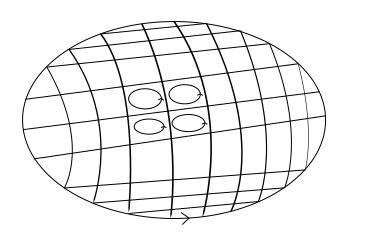
\includegraphics[scale=.5]{trasporto.png}
\caption{Il trasporto parallelo è indipendente dal percorso.}
\label{trasporto}
\end{figure}

Se questo è vero in un punto prendo una base di vettori dello spazio cotangente e li propago parallelamente in questo modo definisco un campo di 1-forme (questo perché il propagatore parallelo non dipende dal loop (anche se lo spazio non è semplicemente connesso?). Inoltre in ogni punto e per ogni direzione $\frac{dx^{\mu}}{d\lambda} \nabla_{\mu} \omega_{\nu} = 0$, dunque $\nabla_{\mu} \omega_{\nu} = 0$ e l forma differenziale definita è chiusa. Su un dominio semplicemente connesso essa è anche esatta: $\omega = df$. Questa funzione $f$ definisce la prima coordinata del nuovo sistema di riferimento e ripeto l'operazione per tutte le coordinate. Il prodotto scalare di due vettori $g(X, Y) = g_p (X_p, Y_p)$ è uguale a quello dei vettori parallelamente trasportati, quindi considerando i vettori di base si vede che la metrica è ovunque Minkowski. Credo che per dimostrare che $Riem = 0 \rightarrow $ trasporto parallelo indipendente dal percorso serva il teorema di Frobenius. 
Negli esempi che fa Carroll per mostrare la differenza tra curvatura intrinseca e curvatura estrinseca si considera sempre una carta locale sai per il toro che per la sfera: con la metrica $g = d\phi^2+d\theta^2$. 

\textbf{Simmetrie e vettori di Killing}
 Se la metrica è invariante per trasformazioni temporali, l'energia è conservata. Nel caso della metrica di Friedman non è così. Ci sono alcune properità utili dei vettori di Killign dimostrate sul Weinberg: $\nabla_{\mu} \nabla_{\sigma} K^{\rho} = R^{\rho}_{\sigma \mu \nu} K^{\nu}$, dalla quale segue: $\nabla_{\mu} \nabla_{\sigma} K^{\rho} =R_{\sigma \nu} K^{\nu}$ e usando l'identità di bianchi (suppongo $\nabla_{[a}R_{bc]de} = 0$ porta all'equazione: $K^{\lambda} \nabla_{\lambda} R = 0$. Notare che essere campo vettoriale di Killing è una richiesta locale.
Bisogna applicare la definzione di tensore di Riemann come commutatore delle derivate covarianti per ricavare questa espressione, che permette a partire dalla conoscenza di $K^{\mu}$ e di $\nabla_{\mu} K^{\nu}$ di trovare tutte le derivate del campo di Killing e dunque di trovare il campo in un aperto. La serie potrebbe coincidere su tutta la carta ma non è detto su tutta la varietà. In particolare tutte le derivate saranno combinazioni lineari di $K^{\mu}$ e di $\nabla_{\mu} K^{\nu}$, pertanto come mostrato sul Weinberg il numero massimo di vettori di Killing è $\frac{n(n+1)}{2}$, poiché vi sono questo numero di modi linearmente indipendenti di scegliere le condizioni iniziali (finire di guardare sul Weinberg).
Se si trova un campo vettoriale di Killing time-like si può costruire una famiglia di superfici $\Sigma_t$ ortogonali al campo massimalmente estese nella direnzione spaziale (credo si possa fare su tutto lo spazio). Un osservatore che si muove lungo le linee integrali del campo di Killing vede queste superfici come lo spazio tridimesionale a tempo costante. Dal teorema di Stokes sappiamo che la quantità: $\int_{\Sigma_t} J^{\mu} n_{\mu} \sqrt{\gamma} d^3x$ è conservata per ogni istante di tempo $t$ (fino a quando si riescono a definire le coordinate normali riemanniane?). Similmente posso usare Killing space-like per costruire momenti conservati.\\



\textbf{Scrivere appunti sui vettori di Killing conformi (su wikipedia è riportato del materiale ma io vorrei riuscire anche ad "esponenziare" quella relazione per trovare che il pullback della metrica rispetto ad un campo di killing conforme è legato con una trasformazione conforme alla metrica originale (credo sia vero) e perché i vettori di Killing formano un'algebra chiusa. Probabilmente facendo esplicitamente il conto viene, cioè mostrare che il commutatore soccisfa l'equazione dei vettori di Killing.}
\textbf{Mostrare che una trasformazione conforme manda geodetiche nulle in geodetiche nulle.}


\textbf{Spazi massimalmente simmetrici}
\textbf{Definizione:} Uno spazio è omogeneo se è invariante per ogni traslazione lungo ogni coordinata. Mentre è isotropo se è invariante per rotazione di una coordinata in un'altra.
Lo spazio con il maggior numero di simmetria ($\frac{n(n+1}{2}$) è $\mathcal{R^{n}}$, in particolare ogni spazio può essere scritto localmente come $\mathcal{R^{n}}$ in coordinate cartesiane, pertanto il numero massimo di simmetrie possibili di uno spaziotempo di dimensione n è: ($\frac{n(n+1}{2}$).

\textbf{Teorema:} IL tensore curvatura di Riemann per uno spazio massimalmente simmetrico è: $R_{\rho \mu \sigma \nu} = \frac{R}{N(N-1)} (g_{\rho \mu} g_{\sigma \nu} - g_{\rho \nu} g_{\sigma \mu})$, dove $R$ è la curvatura scalare costante su tutta la varietà.
(Non penso si possa trattare $\nabla_a$ come un tensore, la derivata covariante è definita come una mappa tra tensori di tipo diverso.)
Passando in coordinate localmente inerziali si può mostrare che: $[\nabla_{\mu}, \nabla_{\nu}] \nabla_{\sigma} V_{\rho} = -R^{\alpha}_{\sigma \mu \nu} \nabla_{\alpha} V_{\rho} + R^{\alpha}_{\rho \mu \nu} \nabla_{\sigma} V_{\alpha}$. 
Si può esprime il membro sinistro usando le due equazioni: 
$\nabla_{\mu} V_{\nu} + \nabla_{\nu} V_{\mu}$ e $\nabla_{\rho} \nabla_{\sigma} V_{\mu} = 
-R^{\lambda}_{\sigma \rho \mu} V_{\lambda}$. Ottenendo: $[\nabla_{\mu} R^{\alpha}_{\nu \sigma
 \rho} - \nabla_{\nu} R^{\alpha}_{\mu \sigma \rho}] V_{\alpha}+[R^{\beta}_{\nu \sigma \rho}
 \delta^{\alpha}_{\mu} -R^{\beta}_{\mu \sigma \rho} \delta^{\alpha}_{\nu} + R^{\alpha}_{\sigma
  \mu \nu} \delta^{\beta}_{\rho} -R^{\alpha}_{\rho \mu \nu} \delta^{\beta}_{\sigma}]
   \nabla_{\alpha}
  V_{\beta} = 0$. 
Se lo spazio è massimalmente simmetrico in ogni punto posso prendere un vettore di Killing che si annulla $V_{\mu} = 0$ e le cui componenti libere di $\nabla_{\mu} V_{\nu}$ sono tutte le possibili $\frac{n(n-1)}{2}$. 
Quindi $R^{\beta}_{\nu \sigma \rho} \delta^{\alpha}_{\mu} -R^{\beta}_{\mu \sigma \rho} \delta^{\alpha}_{\nu} + R^{\alpha}_{\sigma \mu \nu} \delta^{\beta}_{\rho} -R^{\alpha}_{\rho \mu \nu} \delta^{\beta}_{\sigma}$ essere simmetrico. 
Se è è presente il numero massimale di vettori di Killing posso combinarli linearmente in modo che in un certo punto in un sistema localmente inerziale le simmetrie siano le translazioni e le rotazioni. In queste coordinate è evidente che la parte antisimmetrica del tensore sopra scritto è nulla, questa relazione passa a un qualunque sistema di riferimento. 
Scrivendo esplicitamente la simmetria del tensore e contraendo $\alpha$ e $\mu$ (e usando le proprietà del tenore di Riemann) come mostrato sul Weinberg si ottiene la relazione: $R_{\sigma \rho} = \frac{1}{n} g_{\sigma \rho} R$. Dove $R$ è la curvatura scalare. Sostituendo nelle equazioni precedenti contratte (vedi Weinberg) si ottiene la relazione cercata: $R_{\rho \mu \sigma \nu} = \frac{R}{N(N-1)} (g_{\rho \mu} g_{\sigma \nu} - g_{\rho \nu} g_{\sigma \mu})$.
Si può ancora vedere come usando l'identità di Bianchi si possa mostrare che la curvatura scalare è costante su tutto lo spazio. In due dimensioni il Riemnann è sempre nella forma scritta precedentemente, con una curvatura scalare eventualmente non costante.
\textbf{Caratterizzazione degli spazi massimalmente simmetrici}
Gli spazi massimalmente simmetrici sono totalmente caratterizzati (a livello locale) dalla dimensione, dalla segnatura del tensore metrico e dalla curvatura scalare (Carroll) ed eventualmente dalle proprietà topologiche globali (vedi anti de Sitter). Sul Weinberg si trova una dimostrazione di come date due metriche massimalmente simmetriche aventi stessa curvatura scalare si trovi un cambio di coordinate che mostra come siano in realtà la stessa metrica. Gli spazi massimalmente simmetrici possono essere diversi per la topologia globale.
\textbf{Costruzione di spazi massimalmente simmetrici}
La seguente discussione è ripresa dal Weinberg. Sia dato uno spazio $(n+1)$ dimensionale con metrica data da: $ds^2 = C_{\mu \nu} dx^{\mu} d^{\nu} + \frac{1}{K} dz^2$. Considero al sottovarietà definita dalla ipersuperficie $KC_{\mu \nu} x^{\mu} x^{\nu} + z^2 = 1$. La metrica indotta su questa superficie è: $g_{\mu \nu} = C_{\mu \nu} + \frac{K}{(1-KC_{\rho \sigma} x^{\rho} x^{\sigma}} C_{\mu \lambda} x^{\lambda} C_{\nu \epsilon} x^{\epsilon}$. E' ovvio che l'ipersuperficie ammette il numero massimale di isometrie. I simboli di Christoffel possono essere calcolati e forniscono. $\Gamma^{\mu}_{\nu \lambda} = K x^{\mu} g_{\nu \lambda}$. Questo significa che l'equazione geodetica è: $\frac{d^2 x^{\mu}}{dt^2} + K x^{\mu}$, si tratta dell'equazione del moto armonico semplice. La segnatura della metrica $g_{\mu \nu}$ dipende dal carattere della superficie scelta, in particolare se $n^{\mu}$ è la normale all'ipersuperficie il segno "tolto" dalla metrica dello spazio in cui si esegue l'embedding è $g_{\mu \nu} n^{\mu} n^{\\nu}$, se il carattere del vettore si mantiene costante lungo tutta l'ipersuperficie la metrica mantiene la stessa segnatura ovunque.
E' possibile applicare una trasformazione lineare delle coordinate in tutto lo spazio che riporta $C_{\mu \nu}$ alla forma normale (di Sylvetser). 
Applichiamo questa procedura nel caso di uno spazio Euclideo tridimensionale costruito tramite embdedding in uno spazio quadridimensionale Euclideo. La metrica si può scrivere: $ds^2 =dx^2+dy^2+dz^2+\frac{K(\vec{x} \vec{dx})^{2}}{1-K x^2}$. Dalla relazione $r dr = x dx + y dy +z dz$ si può ricavare che la generica forma per una metrica massimalmente simmetrica è: $ds^2 = r^2 d\Omega^2 + \frac{dr^2}{1-k r^2}$. Questa metrica sarà importante per modello FLRW.
\textbf{Spazi di deSitter e di Anti deSitter}
Cerchiamo nello spazio tempo di Minkowski gli spazi MSS a curvatura positiva e negativa (questi sono detti spazi di deSitter e di Anti deSitter (AdS).
Consideriamo $ds^2 = -du^2 + dx^2+ dy^2+dz^2+dw^2$ e in esso la "palla" $-u^2+x^2+y^2+z^2+w^2 = \alpha^2$. Usando la formula di prima si può esprimere il differenziale $dw£$ in termini degli altri quatto e sostituirlo nella metrica sulla in tutto lo spazio per ottenere la metrica sulla ipersuperficie. Verifichiamo che la metrica indotta è lorenziana (vedi Hawking - hypersurfaces). $n_{\mu} = \nabla_{\mu} f$ con $f(u, x, y, z, w) = -u^2+x^2+y^2+z^2+w^2$, dunque $n_{\mu} = 2(-u, x, y, z, w)$. Il modulo di questo vettore e nella metrica ambiente è: $-u^2+x^2+y^2+z^2+w^2$ dunque sempre positivo (per ipotesi) e normalizzabile. Pertanto per trovare la segnatura della metrica sullo spazio di deSitter bisogna togliere alla metrica dell'ambiente un segno +. Parametrizziamo lo spazio con coordinate diverse:

\begin{equation}
   \begin{cases}
   u = \alpha sinh \left( \frac{t}{\alpha} \right) \\
   w = \alpha cosh \left( \frac{t}{\alpha} \right) cos (\chi)\\
   x = \alpha cosh \left( \frac{t}{\alpha} \right) sin (\chi) sin(\theta) \cos(\phi)\\
   y = \alpha cosh \left( \frac{t}{\alpha} \right) sin(\chi) \sin(theta) \cos(\phi)\\
   z = \alpha cosh \left( \frac{t}{\alpha} \right) sin(\chi) sin(\theta) \\
   \end{cases}
\end{equation}

Eseguendo le dovute sostituzioni (farle una volta) si ottiene la metrica $ds^2 = -dt^2 + \alpha^2 cosh^2 \left( \frac{t}{\alpha} \right) [d \chi^2 + sin^2 \chi (d \theta ^ 2 + sin^2 \theta d \phi ^ 2)]$. In queste coordinate lo spazio di deSitter è una 3-sfera che si contrare e poi si espande nuovamente.
Lo spazio di deSitter è chiaramente massimalmente simmetrico perché sia la metrica dello spazio in cui si ha l'embedding sia la sua definizione come iperboloide sono invarianti per il gruppo $O(1,4)$, quindi anche la metrica dello spazio di de Sitter è invariante per questo numero di trasformazioni indipendenti quindi è massimalmente simmetrico.
\textbf{Domanda}: Perché le coordinate date coprono tutta la carta?

Lo spazio di Anti deSitter si ottiene dall'embedding nello spazio 5-dimensionale dotato della metrica fittizia $ds^2 = -du^2 -dv^2 + dx^2 + dy^2 + dz^2$ dell'ipersuperficie $-u^2-v^2+x^2+y^2+z^2 = -\alpha^2$. Ripetendo l'analisi del paragrafo precedente si vede come il vettore $n^{\mu}$ abbia modulo $-u^2-v^2+x^2+y^2+z^2 = -\alpha^2$ dunque sempre negativo e per ottenere la segnatura della metrica sull'ipersuperficie bisogna togliere un -. Cambiando coordinate come indicato da Carroll si incorre nella necessità di dover definire lo spazio di Anti deSitter come ricoprimento universale, spazi con la stessa metrica possono differire sulla topologia globale. Questi spazi sono soluzioni dell'equazione di Einstein per un universo vuoto con constante cosmologica rispettivamete positiva e negativa.

\textbf{Topologia degli spazi di deSitter e Anti deSitter (ancora da capire)}
Lo spazio di deSitter è topologicamente $R \times S^3$, mentre quello di Anti deSitter è $\mathcal{R^{n}}$. Le coordinate introdotte per questi spazi lo coprono tutto con una sola carta, questo si può verificare studiando le geodetiche e vedendo che non si interrompono per un valore finito del parametro affine. Non mi è chiaro quali costrizioni topologiche da la metrica in generale?.

\textbf{Metrica di Robertson-Walker}
L'assunzione del Principio Cosmologico per l'universo dovrebbe essere massimalmente simmetrico è contraddetta dall'esperienza infatti l'assunzione Standard è che l'universo sia una varietà del tipo $\mathcal{R} \times \Sigma$ dove $\Sigma$ è una 3-varietà massimalmente simmetrica secondo la metrica globale indotta. Spazi MS che localmente (su un aperto) hanno la stessa e metrica e sono isomorfi possono differire per le proprietà globali e non è detto che $\Sigma$ sia $\mathcal{R^{3}}$. L'introduzione della coordinata $d \chi = \frac{dr}{\sqrt{1-Kr^2}}$ permette di riscrivere la metrica spaziale come:

\begin{equation}
	\begin{cases}
	d \sigma ^ 2 = d \chi^2 + sin(\chi)^2 d \Omega^2 (K < 0)\\
	d \sigma ^ 2 = d \chi^2 + \chi^2 d \Omega^2 (K = 0)\\
	d \sigma ^ 2 = d \chi^2 + sinh(\chi)^2 d \Omega^2 (K > 0)\\	
	\end{cases}
\end{equation}

L'informazione sulla metrica di essere massimalmente simmetrica è solamente locale (si riferisce alle derivate di Lie in ogni punto). Essendo in ogni punto la metrica lorenziana su $\mathcal{R^{4}}$ possiamo pensare che non possa avere più vettori di Killing della metrica di Minkowski stessa. Tuttavia conoscere la metrica in una certa carta (che può coprire o meno tutta la varietà, non vuol dire conoscere la topologia e la metrica piatta potrebbe essere su $\mathcal{R^{3}}$ oppure su $S^{1} \times S^{1} \times S^{1}$ (Assumendo che lo spazio tempo sia fogliabile come $S^{1} \times \Sigma$. Analogamente possiamo immaginare che la metrica dello spazio chiuso sia quella di una sfera e quella dello spazio aperto sia un'iperboloide (non compatto), tuttavia possiamo avere la merica FLRW aperta anche su una varietà non semplicemente connessa ma compatta 3D, in questo caso vale l'ipotesi di semplicità che lo spazio sia semplicemente connesso.

\textbf{Domanda:} tutte e sole le soluzione dell'equazione di Einstein nel vuoto con costante cosmologica sono massimalmente simmetriche?

Si possono costruire gli SMS tramite embedding in spazi di dimensione maggiore con diverse metriche possibili, considerando le sfere del tipo $\-t^2+x^2+y^2+z^2+w^2 = \alpha^2$ bisogna fare in modo che la metrica indotta sulla sottovarietà sia della segnatura desiderata (vedi Hawking). Queste sottovarietà hanno naturalmente il numero desiderato di simmetrie e si può mostrare che in generale hanno il Riemann dato da: $R = \frac{R}{N(N-1)} (g_{\rho \mu} g_{\sigma \nu} - g_{\rho \nu} g_{\sigma \mu})$ (vedi tesi di TorVergata e Weinberg). Vedi $\href{https://physics.stackexchange.com/questions/99882/how-to-prove-that-a-spacetime-is-maximally-symmetric/99975#99975}{StackExchange}$.

\textbf{Spin connection and vielbein}
Scrivere parte sulle connessioni e sulle vielbein. Non capisco perché il tensore di Riemann è una (1,1)-valued 2-form mentre nella teoria quantitica di Yang e Mills essa sarebbe solo una (1,0) valued 2-form.

\textbf{Formalismo ADM e energia gravitazionale.}

\textbf{13 Agosto - Pausa relatività generale per studiare teorica 1.}

\textbf{Question asked on stack exchange}
In general relativity the fourvelocity of a timelike particle following a path $x^{\mu}(\tau)$ is defined as the derivative $u^{\mu} = \frac{dx^{\mu}}{d \tau}$ where $\tau$ is the proper time of the curve, i. e. $\tau = \int_{\lambda_0}^{\lambda_1} \sqrt{g_{\mu \nu} \frac{dx^{\mu}}{d \lambda} \frac{dx^{\nu}}{d \lambda}}$ where $\lambda$ is an arbitrary parametrization of the curve. Among all the possible affine parameters the preferred one is the proper time for which we define the fourvelocity. Similarly for a space-like curve the preferred affine parameter is the "lenght" of the curve, however we wouln't call the derivative of the coordinates with respect to such parameter a fourvelocity. For nulllike geodesics there no preferred choise of the affine parameter, it still make sense to \textbf{define} the fourmomentum as $p^{\mu} = \frac{dx^{\mu}}{d \lambda}$ but how can we fix the multiplicative constant which can arise from $\lambda \rightarrow a \lambda$ which gives $p'^{\mu} = \frac{dx^{\mu}}{d (a \lambda)} = \frac{1}{a} p^{\mu}$? It sees to me that it cannot be done in this context and one should impose the correct fourmomentum "by hand".
La risposta è che si può sempre scegliere un parametro affine che permette di fissare la "qudrivelocità" con cui viene percorsa la curva al quadrimomento fisico del fotone, bisogna quindi cercare la parametrizzazione che da la fisica corretta.

\textbf{Soluzione di Schwarzschild}
Data la metrica in coordinate di Schwarzschild introduco il cambiamento di coorinate per passare alle coordinate di Kruskal. In queste nuove coordinate si potrebbe calcolare il tensore $R_{\mu \nu \rho \sigma}$ che sapremmo essere 0 per tutti i $T$, $R$ che corrispondono alla metrica di Schwarzschild. Tuttavia esso è 0 anche per gli altri valori di $T$, $R$ che non finiscono sulla singolarità della metrica a $r=0$ quindi abbiamo una soluzione massimalmente estesa (si può dimostrare che è massimale?) della metrica a simmetria sferica stazionaria (anche statica).

\end{document}